\documentclass[twocolumn]{article}

\usepackage[T1]{fontenc}
\usepackage[utf8]{inputenc}
\usepackage[spanish]{babel}
\usepackage{microtype}
\usepackage{lipsum,blindtext}
\usepackage{abstract}     
\usepackage{graphicx}
\usepackage{booktabs}
\usepackage{hyperref}
\usepackage{float}

\hypersetup{colorlinks=true, urlcolor=blue, linkcolor=black, citecolor=black}

\usepackage[style=apa,backend=biber]{biblatex}
\DeclareLanguageMapping{spanish}{spanish-apa}
\addbibresource{refs.bib}

\newcommand{\keywords}[1]{\par\noindent\textbf{Palabras clave:} #1}

\title{Robustez y resilencia de la red comparativa}
\author{
    Mathias Hualtibamba, Giorgio Mancusi y Fabio Osorio \\
    Universidad Peruana de Ciencias Aplicadas \\
    Curso: Complex Networks \\
    2025-2 
}
\date{12 de octubre de 2025}

\begin{document}

\maketitle

\begin{abstract}
\blindtext[1]
\keywords{redes complejas, comparativas, analisis de resilencia, grafos}
\end{abstract}

\section{Introduccion}
\blindtext[2]

\section{Marco Teorico}
\subsection{Redes Complejas}
Segun \cite{ding2025comprehensivesurveyartificialintelligence}, las redes complejas constituyen una repsentacion abstracta de sistemas reales formados por multiples componentes interconectados. 
Este tipo de redes puede describir entre los reacciones quimicas hasta las conexiones entre paginas web. Su estudio permite indentificar patrones globales de comportamiento a nivel macro, como las formacion de comunidades o estructuras, mientras que a nivel micro reflejan el desorden y heterogeneidad característicos de los sistemas reales.

\subsection{Grafos}
Según \textcite{Zamora_L_pez_2024}, un grafo es una estructura matemática compuesta por un conjunto de vértices (o nodos) y un conjunto de aristas (o enlaces) que representan las relaciones entre dichos vértices. 
Los grafos permiten modelar y analizar sistemas reales de manera abstracta, facilitando su descripción formal y cuantitativa. 
A través de la teoría de grafos, es posible identificar la arquitectura oculta de un sistema complejo, estudiar sus propiedades estructurales y comprender su comportamiento global. 
Matemáticamente, un grafo puede representarse mediante una matriz de adyacencia, donde cada elemento $a_{ij}$ indica la existencia (y, en redes ponderadas, la intensidad) de la conexión entre los nodos $i$ y $j$.

\section{Metodologia}
\subsection{Datos}
El conjunto de datos utilizado está conformado por seis columnas: \textit{Año}, \textit{Persona}, \textit{Tipo de servicio}, \textit{Nombre de la tarea}, \textit{Modalidad} y \textit{Complejidad}. 
El dataset cuenta con un total de 10,384 registros, de los cuales aproximadamente 3,600 correspondían a duplicados. 
Estos registros fueron eliminados durante la etapa de limpieza, dado que no aportaban información adicional a la estructura del grafo y su presencia incrementaba innecesariamente el costo computacional en la construcción y análisis de la red. 

\subsection{Analisis Exploratorio de los datos - EDA}
Despues de eliminar los 3,600 registros duplicados, se observó que las columnas \textit{Tipo de servicio} y \textit{Nombre de la tarea} presentaban la siguiente distribución:

\begin{figure}[H]
    \centering
    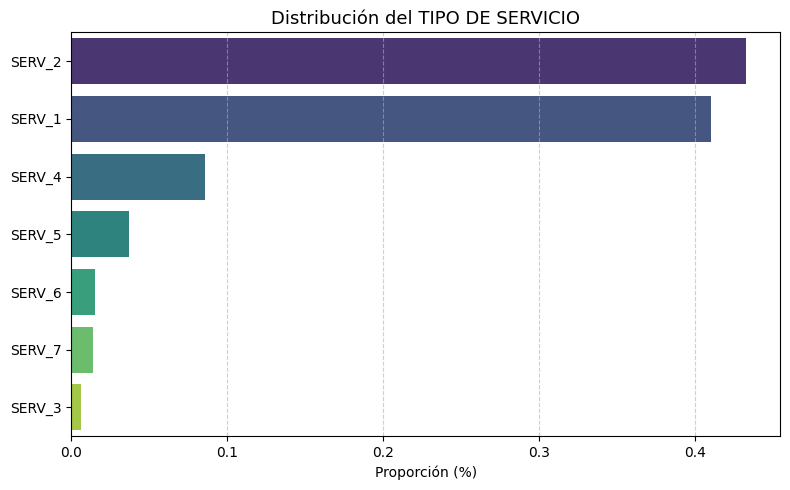
\includegraphics[width=\columnwidth]{img/DistribucionTipoServicio.png}
    \caption{Distribución del TIPO DE SERVICIO.}
    \label{fig:distribucion_tipo_servicio}
\end{figure}

Los servicios \textit{1} y \textit{2} concentraron la mayor parte de los datos, representando aproximadamente el 40\% cada uno, como se muestra en la Figura~\ref{fig:distribucion_tipo_servicio}.

\begin{figure}[H]
    \centering
    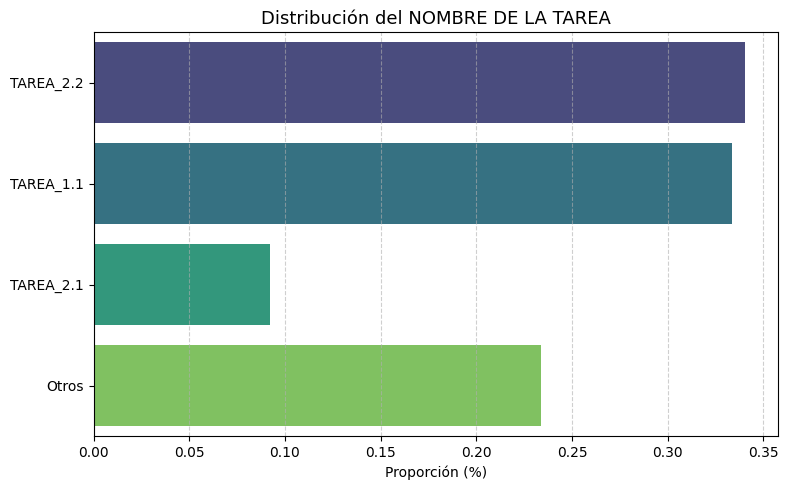
\includegraphics[width=\columnwidth]{img/DistribucionNombreTarea.png}
    \caption{Distribución del NOMBRE DE LA TAREA (80\% + Otros).}
    \label{fig:distribucion_nombre_tarea}
\end{figure}

De manera similar, las tareas \textit{2.2} y \textit{1.1} representaron alrededor del 30\% cada una, como se observa en la Figura~\ref{fig:distribucion_nombre_tarea}.

\begin{figure}[H]
    \centering
    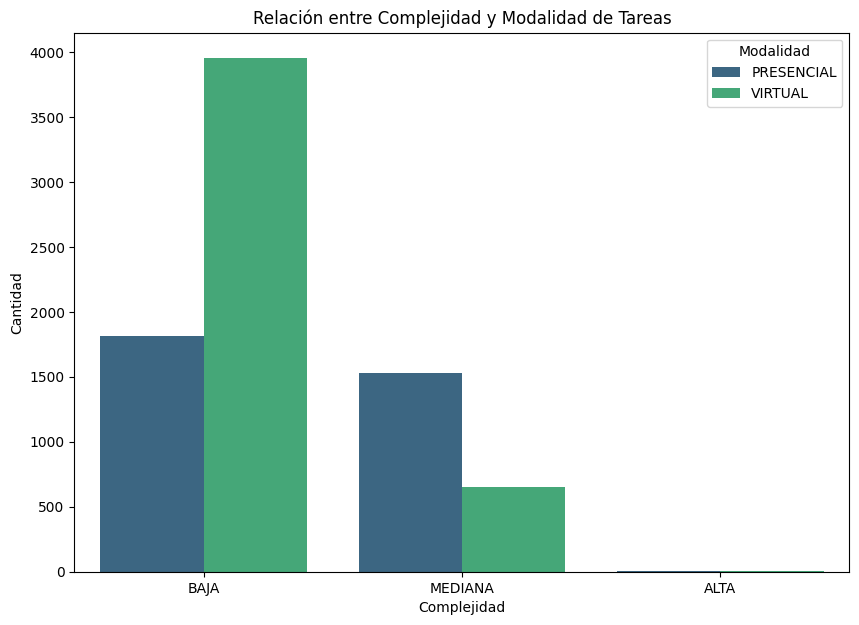
\includegraphics[width=\columnwidth]{img/RelacionComplejidadModalidad.png}
    \caption{Relacion entre Complejidad y Modalidad}
    \label{fig:relacion_complejidadymodalidad}
\end{figure}

Por otro lado, la relación entre la \textit{complejidad} y la \textit{modalidad} de las tareas mostró que las tareas de baja complejidad en modalidad virtual concentraron la mayor proporción del conjunto de datos, como se aprecia en la Figura~\ref{fig:relacion_complejidadymodalidad}.

\subsection{Construccion de la red}
\blindtext[1]

\subsection{Analisis y Metricas}
\blindtext[1]

\subsection{Herramientas}
Las herramientas utilizadas para la creacion del grafo fueron los siguentes:
\begin{itemize}
    \item Python 3.13
    \item NetworkX
    \item Pandas
    \item VSCode
\end{itemize}

\section{Resultados}
\blindtext[4]

\printbibliography

\section{Anexos}
El codigo, notebook y datos se encuentran en el siguente repositorio \parencite{repoCodigo}

\end{document}
